\documentclass[11pt]{article}
\usepackage{graphicx}
\graphicspath{ {./images/} }

\usepackage{algorithm}
\usepackage{algpseudocode}
\usepackage{hyperref}

\usepackage{sectsty}
\usepackage{graphicx}
\usepackage[font=small,labelfont=bf]{caption} % Required for specifying captions to tables and figures

% Margins
\topmargin=-0.45in
\evensidemargin=0in
\oddsidemargin=0in
\textwidth=6.5in
\textheight=9.0in
\headsep=0.25in

% norm function
\newcommand{\norm}[1]{\left\lVert#1\right\rVert}

\title{ %

\includegraphics[width=0.4\textwidth]{UniCT-Logo-Nero}~\\
Trashbin Triplet Classifier \\ 
\large Progetto Deep Learning (LM-18) \\ Università degli Studi di Catania - A.A 2021/2022 \\
}
\author{ Danilo Leocata \\ Docente: Giovanni Maria Farinella, Antonino Furnari}
\date{\today}

\begin{document}

\maketitle	
\pagebreak

%--Paper--

\section{Introduzione}

L'obbiettivo del progetto è realizzare una rete siamese su un dataset di secchi della spazzatura, per classificarne la capienza rimamente e che in particolare sia in grado di distinguere tra: pieno, vuoto, a metà.
Il dataset è stato preso da un precedente progetto (\href{https://github.com/khalld/trashbin-classifier}{repository Github}) in cui è stato allenato un modello che ne classifica la pienezza. Il dataset è disponibile \href{https://drive.google.com/drive/folders/11SGtZrM8BWJDPOcnKR7RjLJs0dJOfSCA?usp=sharing}{al seguente indirizzo}.

Il progetto è stato sviluppato utilizzando \texttt{python v3.9.9} e \texttt{pytorch-lighting v1.6.3}. Il modello è stato allenato utilizzando un MacBook Pro (16-inch, 2019) con processore Intel(R) Core(TM) i7-9750H CPU @ 2.60GHz, ram: 16 GB 16 GB 2667 MHz DDR4 e GPU AMD Radeon Pro 5300M 4 GB
Intel UHD Graphics 630 1536 MB. Sfortunatamente, ad oggi, il modello di GPU non è supportato per l'accelerazione del training e di conseguenza è stato effettuato su CPU.

La repository del progetto è disponibile al \href{https://github.com/khalld/triplet-trashbin-classifier}{seguente} indirizzo.

\section{Scelta dell'architettura}

È stato trovato opportuno l'utilizzo di una \textit{Rete Triplet} per il raggiungimento dell'obbiettivo assegnato, dato che il dataset è composto da 3 classi, è stato pensato che questo approccio sarebbe stato migliore per dare una netta 'differenza' tra la classe 'mezzopieno' e 'vuoto' e 'pieno' (scrivi meglio).
Ogni tripletta $(I_i, I_j, I_k)$ contiene dunque tre elementi

\begin{center}
    \begin{minipage}{0.48\linewidth}
    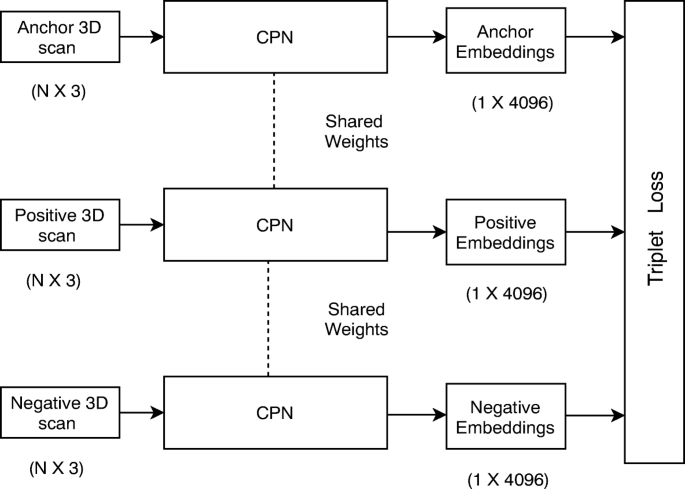
\includegraphics[width=\linewidth]{tripletNetwork.png}
    \end{minipage}
    % \captionof{figure}{Architettura rete neurale triplette} TODO:
\end{center}

\begin{itemize}
    \item L'ancora $I_i$ 
    \item L'esempio positivo $I_j$ (che in breve ha la stessa classe di $I_i$)
    \item L'esempio negativo $I_k$, cioé un elemento diverso dalle classi di $I_i$, $I_j$
\end{itemize}

La coppia $I_i$, $I_j$ sarà un esempio positivo, e la coppia $I_i$, $I_k$ esempio negativo: $I_i$ verrà mappato vicino a $I_j$ e lontano da $I_k$, offrendo sempre un esempio positivo e uno negativi relativo allo stesso elemento.

% TODO:
\textit{
    By enforcing the order of distances, triplet loss models embed in the way that a pair of samples with same labels are smaller in distance than those with different labels. Unlike t-SNE which preserves embedding orders via probability distributions, triplet loss works directly on embedded distances. Therefore, in its common implementation, it needs soft margin treatment with a slack variable 
    $\alpha$  in its hinge loss-style formulation. It is often used for learning similarity for the purpose of learning embeddings, such as learning to rank, word embeddings, thought vectors, and metric learning.
}

\section{Preparazione del dataset}

Si è presentata la necessità di riadattare il dataset in triplette: ad ogni elemento di ancora verrà associato un elemento positivo ed uno negativo, che sarà scelto randomicamente in base alle due classi disponibili (ad esempio, se l'ancora appartiene alla classe 'vuoto', l'elemento negativo sarà 'pieno' o 'mezzo')
Per questo, sono state implementate delle funzioni ad-hoc il cui utilizzo è documentato su \texttt{dataset.ipynb}. 

\begin{center}
    \begin{minipage}{0.48\linewidth}
    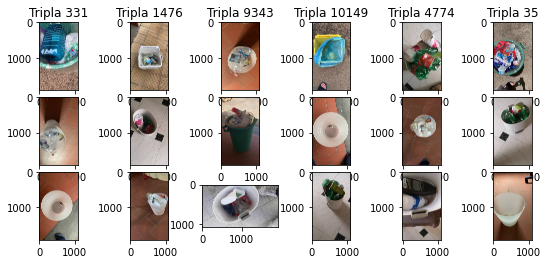
\includegraphics[width=\linewidth]{triplet_dataset.png}
    \end{minipage}
    % \captionof{figure}{Architettura rete neurale triplette} TODO:
\end{center}

Si nota che per incrementare la generalizzazione, sarebbe utile avere a disposizione diversi \texttt{.csv} del dataset adattato ed alternare le varie versioni del dataset dopo un tot di epoche, 
in quanto la funzione è stata implementata in modo tale che le triplette generate siano diverse ad ogni esecuzione del codice.

Partendo dal dataset originale, si è avuta la necessità di riadattarlo in triplette per farlo funzionare per il modello scelto: ad ogni elemento di ancora verrà associato un elemento positivo ed uno negativo che sarà scelto randomicamente in base alle due classi disponibili (esempio: se l'ancora è 'vuoto', l'elemento negativo sarà 'pieno' o 'mezzo')
È stato trovato più efficiente, principalmente per effettuare le prove, 'fissare' il dataset in un \texttt{csv}, evitando di creare le triplette dinamicamente. Per generalizzare ancora di più, sarebbe utile eseguire il codice di creazione del dataset più volte e cambiare il datamodule durante il load del checkpoint: infatti .sample() utilizzato pescherà randomicamente dal dataframe un elemento randomico: in questo modo vi è improbabile che le triplette generate siano uguali ad altre.

\section{Implementazione della rete neurale}

\subsection{Scelta del modello}

\begin{center}
    \begin{minipage}{0.48\linewidth}
    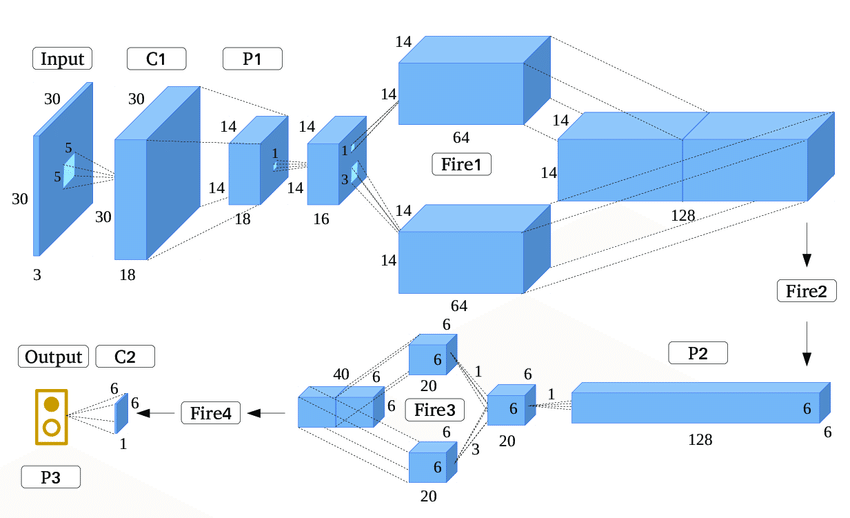
\includegraphics[width=\linewidth]{SqueezeNet-like-architecture.png}
    \end{minipage}
    % \captionof{figure}{Architettura squuezeNet like} TODO:
\end{center}

Nel progetto precedente, sono stati presi in esame alcuni modelli pretrained, utilizzandoli come feature extraction sono stati ottenuti dei buoni risultati in un tempo relativamente breve.
Di conseguenza, nonostante la differenza di potenza computazionale a disposizione, rispetto al precedente progetto, è stato trovato opportuno utilizzare \texttt{SqueezeNet v1} come feature extractor, che aveva comunque dato il miglior risultato in termini di tempo di esecuzione e validazione.

Ad esempio, il completamento di un'epoca utilizzando \texttt{MobileNetV2} richiedeva 1h e 10 minuti contro i 35/40 di \texttt{SqueezeNet v1}. Approssimando, utilizzando immagini a colori 224x224 ed effettuando un training di 60 epoche utilizzando \texttt{SqueezeNet v1} impiegherebbe 30 ore contro le 70 di \texttt{MobileNetV2}.

% TODO: È stato visto (dove?? link???) e testato che nel metric learning, batch più grandi possono portare ad una migliore generalizzazione di batch piccoli, oltre a ridurre di poco il tempo durata del training, di conseguenza dopo varie prove effettuate

\subsection{Ottimizzazione dei parametri}

Sono state sfrittate tecniche di training, già implementate su \texttt{pytorch-lighting}, per ottimizzare il training del modello. In particolare:

\begin{itemize}
    % TODO: traduci e spiega a cosa serve
    \item \textbf{Batch Size Finder} Auto-scaling of batch size can be enabled to find the largest batch size that fits into memory. Large batch size often yields a better estimation of the gradients, but may also result in longer training time
    % TODO: traduci e spiega a cosa serve
    \item \textbf{Learning Rate Finder} For training deep neural networks, selecting a good learning rate is essential for both better performance and faster convergence. Even optimizers such as Adam that are self-adjusting the learning rate can benefit from more optimal choices. To reduce the amount of guesswork concerning choosing a good initial learning rate, a learning rate finder can be used. As described in this paper a learning rate finder does a small run where the learning rate is increased after each processed batch and the corresponding loss is logged. The result of this is a lr vs. loss plot that can be used as guidance for choosing an optimal initial learning rate.
\end{itemize}

\section{Scelta della loss}

Per il training della rete siamese sono state prese in esame due loss differenti

\subsection{Triplet margin loss}
Dati in input i tensori $x_1$, $x_2$, $x_3$ e il margine con un valore più grande di zero.
Questa è usata per misurare una similitudine tra i samples. Una tripletta è composta da a, p ed n. La shape dovrebbe essere (N,D)
La funzione di loss per ogni sample nel mini-batch è:


\begin{center}
    \ \
    $L(a,p,n) = \max{ \{ d(a_i, p_i) - d(a_i, n_i) + margin, 0 \} }$, dove
    \\
    $d(x_i, y_i) = \|| x_i - y_i ||\ _p$
    \ \
\end{center}

\subsection{Triplet margin with distance loss}
Misura la triplet loss dati in input i tensori $a$, $p$ ed $n$ (rispettivamente un esempio ancora, positivo e negativo) ed una funzione a valori
reali non negativa chiamata 'funzione di distanza' usata per calcolare la relazione tra l'ancora e l'esempio positivo (distanza positiva) e l'ancora e l'esempio negativo (distanza negativa)

La loss non ridotta può essere descritta dalla seguente formula:

\begin{center}
    $l(a,p,n) = L = { \{ l_1, \ldots, l_N \}}^T, l_i = \max{\{ d(a_i, p_i) - d(a_i, n_i) + margin, 0 \}} $
\end{center}

Dove N è la dimensione del batch, d è una funzione non negativa a valori reali che quantifica la vicinanza di due tensori riferito alla funzione di distanza,
ed il margine è un margine non negativo che rappresenta la differenza minima tra le distanze positive e negative che è richiesta dalla loss sia 0.
Il tensore di input ha N elementi ognuno del quale può essere di qualsiasi forma che la funzione di distanza può gestire.

Di default come funzione di distanza è stata utilizzata la paiwrise distance funtion che calcola la distanza tra i vettori $v_1$ e $v_2$ usando la p-norm:

\begin{center}
    $ \| x \| _p = ( \sum^n_{i=1} |x_i|^p )^{\frac{1}{p}} $
\end{center}

Effettuando delle prove utilizzando un dataset senza data augmentation 


\section{Training}

Il codice utilizzato per effettuare il training è presente su \texttt{main.ipynb}
Prima di procedere con il training del modello, per mezzo della funzione \texttt{evaluate performance} sarà possibile di predire le etichette sul test set usando Nearest Neighbor, la cui bontà è ottenuta misurando la distanza euclidea tra i valori di label predetti e quelli di ground truth. \textit{Successivamente le rappresentazioni spaziali saranno plottate su un grafico utilizzando il TSNE}.

Nonostante le loss diverse, i due modelli, prima del training, ottengono lo stesso errore di classificazione: \texttt{6.855654600401044}. 
Alla fine del training l'errore di classificazione, sarà \texttt{2.449489742783178}. Le reti sono state allenate per 30 epoche in totale, il grafico di output è il seguente





\begin{center}
\begin{minipage}{0.48\linewidth}
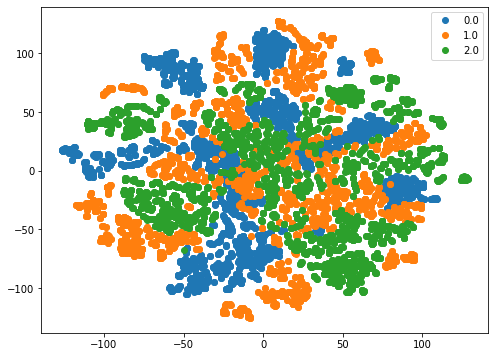
\includegraphics[width=\linewidth]{output_squeezeNet_v1_0epoch.png}
\end{minipage}%
\begin{minipage}{0.49\linewidth}
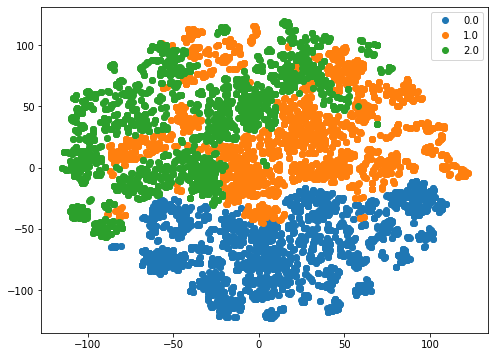
\includegraphics[width=\linewidth]{output_squeezeNet_v1_10epoch.png}
\end{minipage}
\begin{minipage}{0.49\linewidth}
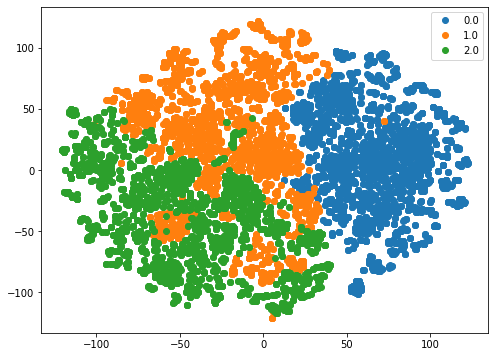
\includegraphics[width=\linewidth]{output_squeezeNet_v1_30epoch.png}
\end{minipage}
\captionof{figure}{Rappresentazioni estratte dopo 0, 10 e 30 epoche}
\end{center}

\begin{center}
    \begin{minipage}{0.48\linewidth}
    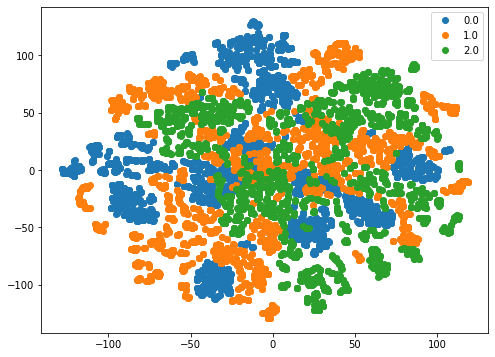
\includegraphics[width=\linewidth]{output_squeezeNet_v2_0epoch.png}
    \end{minipage}%
    % \begin{minipage}{0.49\linewidth}
    % \includegraphics[width=\linewidth]{output_squeezeNet_v2_10epoch.png}
    % \end{minipage}
    \begin{minipage}{0.49\linewidth}
    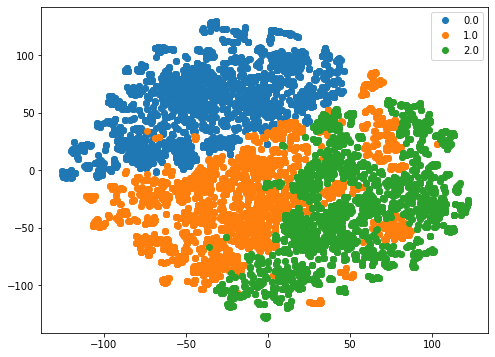
\includegraphics[width=\linewidth]{output_squeezeNet_v2_30epoch.png}
    \end{minipage}
    \captionof{figure}{Rappresentazioni estratte prima del training e dopo 30 epoche}
\end{center}


\begin{center}
    \begin{minipage}{0.48\linewidth}
    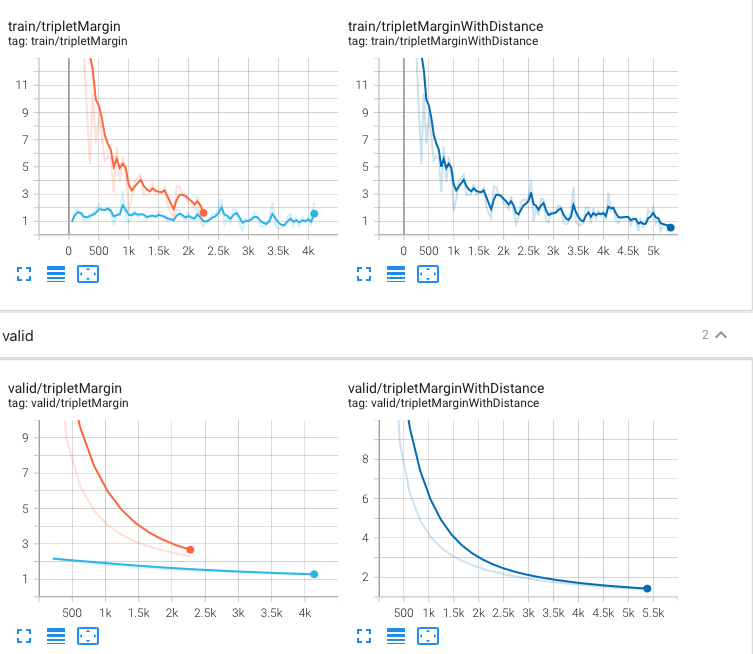
\includegraphics[width=\linewidth]{tensorboard_1.png}
    \end{minipage}
    % \captionof{figure}{Rappresentazioni estratte prima del training e dopo 30 epoche}
\end{center}

\begin{center}
    \begin{minipage}{0.48\linewidth}
    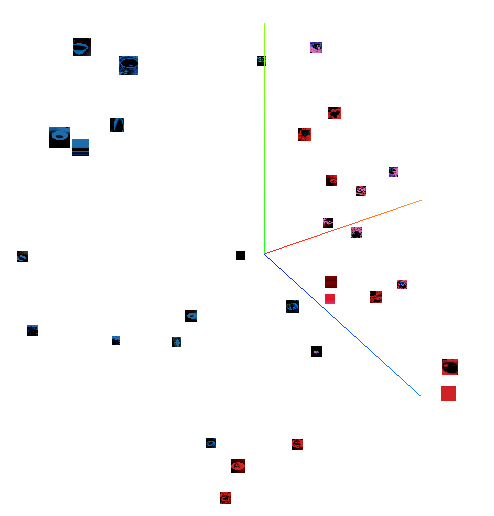
\includegraphics[width=\linewidth]{tensorboard_2.png}
    \end{minipage}
    % \captionof{figure}{Rappresentazioni estratte prima del training e dopo 30 epoche}
\end{center}


\pagebreak

% \begin{thebibliography}{5}


% \bibitem{1} \href{https://www.researchgate.net/publication/242463011_An_Effective_Algorithm_for_Minimum_Weighted_Vertex_Cover_problem}{An Effective Algorithm for Minimum Weighted Vertex Cover Problem}
% \bibitem{2} \href{https://www.sciencedirect.com/science/article/abs/pii/S0377221720300278}{A memory-based iterated local search algorithm for the multi-depot open vehicle routing problem}

% \end{thebibliography}


\pagebreak
%--/Paper--

\end{document}
